\documentclass[../main.tex]{subfiles}
\begin{document}

\section{The Schelling Model}

\label{sec:appendix_schelling}

Consider a stylized example of Schelling's residential model: 
An $N \times N$ matrix $\textbf{M}$ represents possible residential locations. Two types af agents $b, r$, graphically depicted as blue and red, respectively, are initially allocated a random location within this grid. Agents can differ in terms of ethnicity, income, culture etc. 

The ratio between the two types of agents is constant $N_{b/r} = \frac{N_b}{N_r}$. Further, a constant share of residential locations are vacant, such that $N_{vacant} = N^2 - (N_b + N_r)$. 

Each agent $i = b, r$ "optimizes" their residential location by the share, $s_i$, of their nearest neighbors, who is of the same type. That is, for $s_i \leq \tau$, where a $\tau$ is a fixed global tolerance parameter for the maximum share of neighbours of a different type, each agent $i$ will move until this condition is satisified. 

This is a somewhat stylized version of the Schelling model, though it accurately depicts the model dynamics... Something about the Schelling model... 

Below is a parameterization of the model described above such that red(?) is always in the minority\footnote{This implementation closely follows \textcite{luca_mingarelli}, who very kindly made his code publicly available.}:

\begin{table}[H]
    \centering
    \caption{Schelling model parameters}
    \begin{tabular}{lc}
    \toprule
      Parameter & Value \\
    \midrule
      $N$         & 100 \\
      $N_r$       & 1.25 \\
      $N_{vacant}$ & 0.1 \\
    \bottomrule
    \end{tabular}
\end{table}

For agents $i, j$, suppose they are numerically represented as $i_{red}=1$, $j_{blue} = 0$ with vacant locations $m_v=-1$ in $\textbf{M}$. We can perform element-wise multiplication and summation for each agent in $M$ to determine whether or not this satisfies the condition $s_i \leq \tau$. This process is called convolution and the operation can be done via the following kernel $\mathbf{K}$:

\begin{lstlisting}[style=pythonstyle]
import numpy as np
KERNEL = np.array([[1,1,1,1,1],
                   [1,1,1,1,1],
                   [1,1,0,1,1],
                   [1,1,1,1,1],
                   [1,1,1,1,1]])

\end{lstlisting}

With the convolution operation defined as:

\begin{equation}
(K \star M)_{i, j}=\sum_{\substack{a \in\left\{-k_x, \ldots, k_x\right\} \\ b \in\left\{-k_y, \ldots, k_y\right\}}} K_{a+k_x, b+k_y} M_{i+a, j+b}
\label{eq:convolution}
\end{equation}

Where $k_x, k_y \in \mathbb{N}_0$. 


That is, I am considering the $k=24$ nearest neighbors in reference to the tolerance parameter $\tau$.

\begin{figure}[H]
\centering
\caption{Schelling model simulations}
	\begin{subfigure}{0.45\textwidth}	
	\centering
    \caption{Integrated society, $1-\tau = 0.25$}
	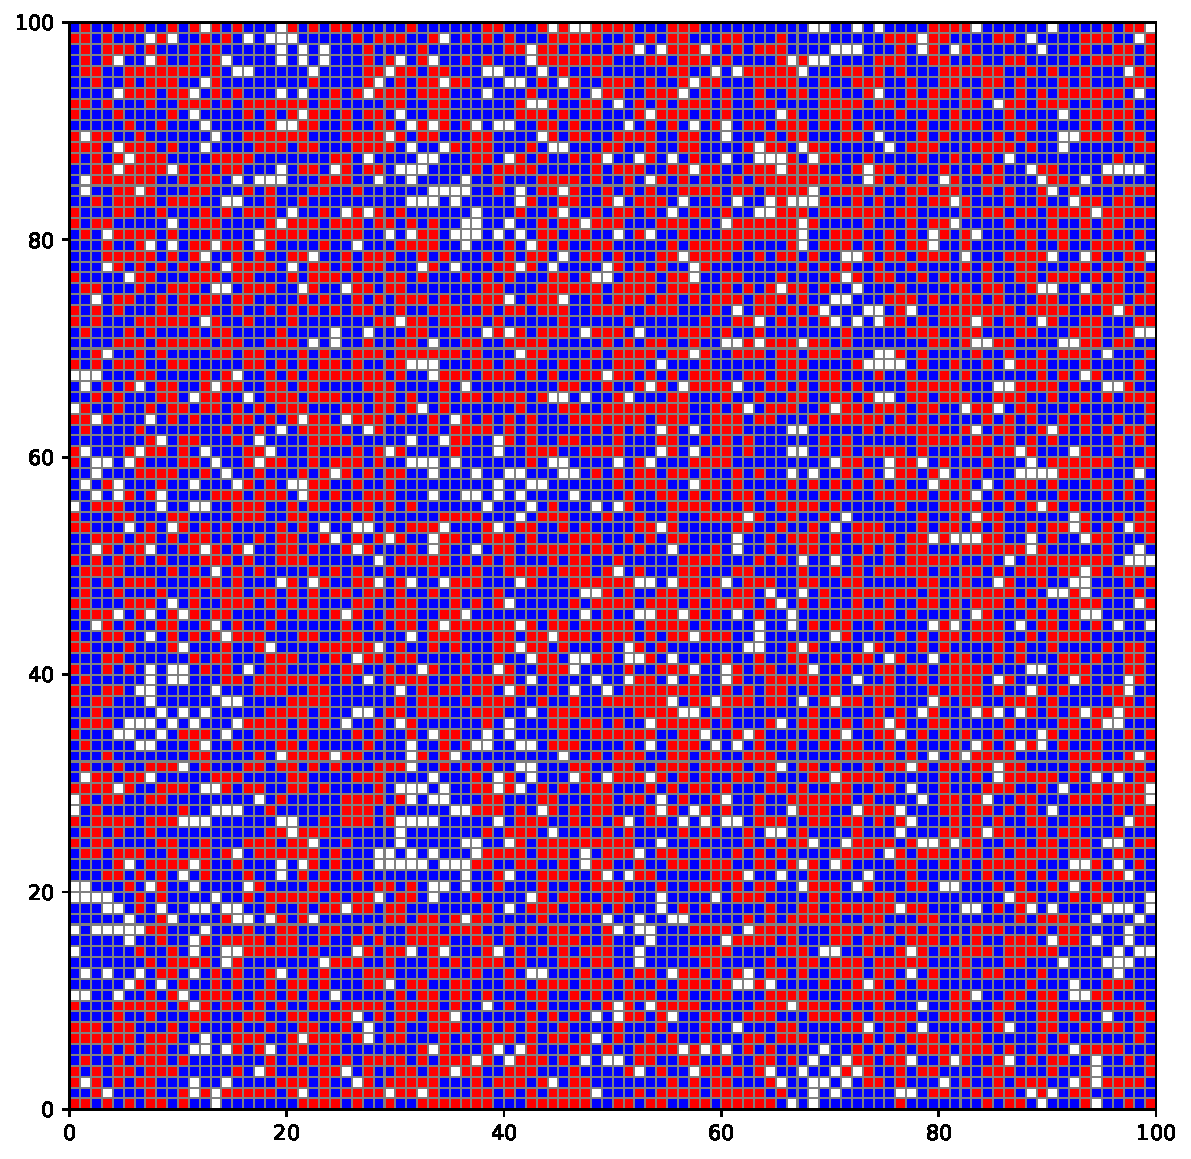
\includegraphics[width=\textwidth]{figs/schelling_model_0.25.pdf}	
	\end{subfigure}	
	\begin{subfigure}{0.45\textwidth}	
	\centering
    \caption{Inbetween(?) society, $1-\tau = 0.33$}
	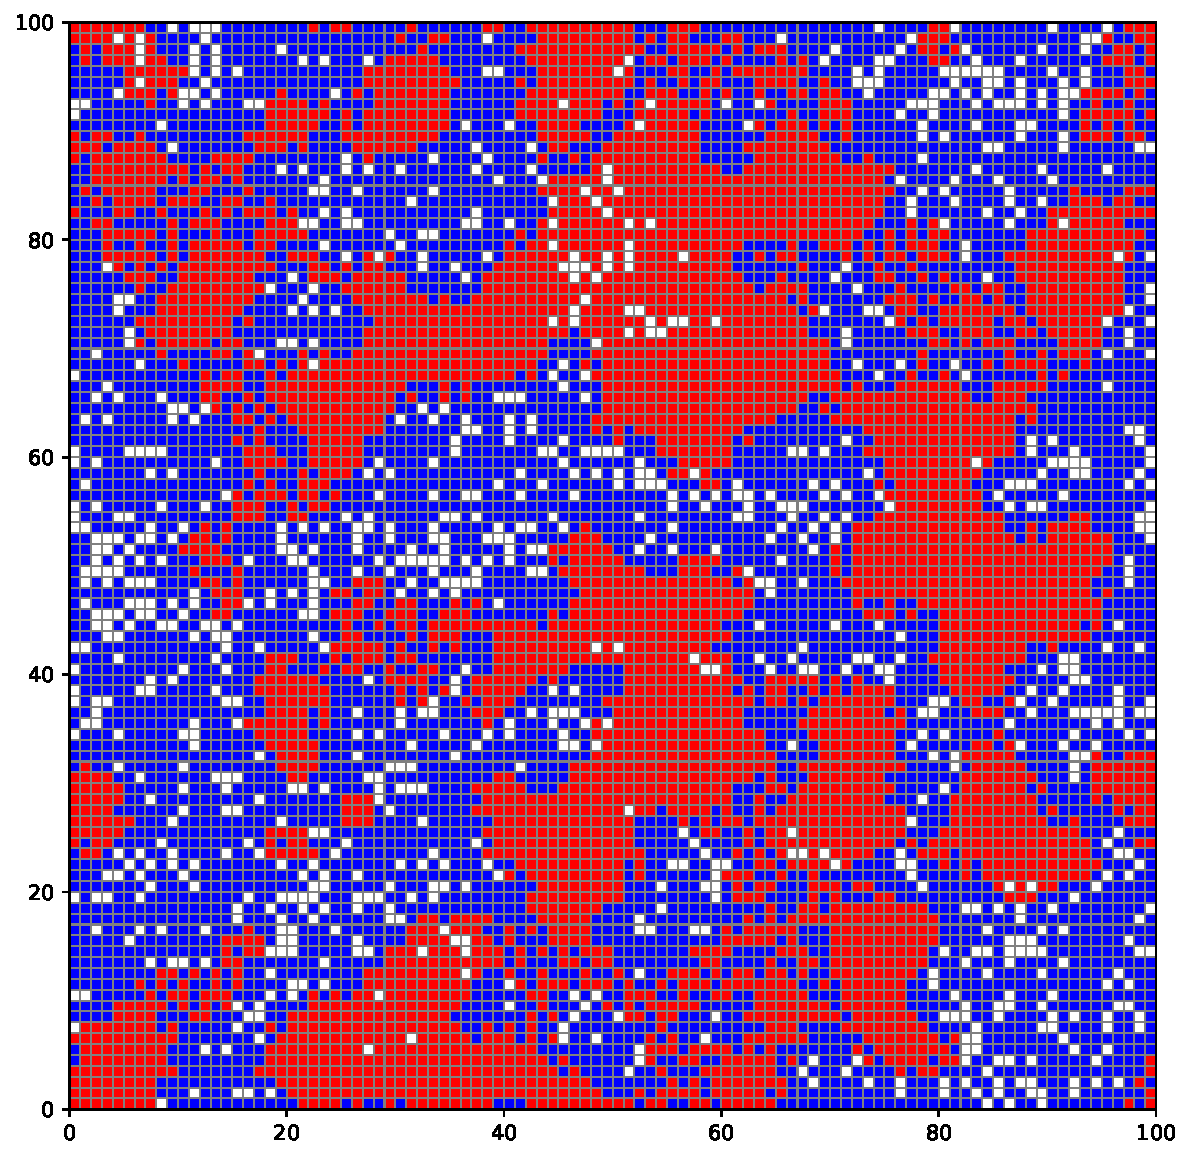
\includegraphics[width=\textwidth]{figs/schelling_model_0.33.pdf}	
	\end{subfigure}	
	\begin{subfigure}{0.45\textwidth}	
	\centering
     \caption{Segregated society, $1-\tau = 0.40$}
	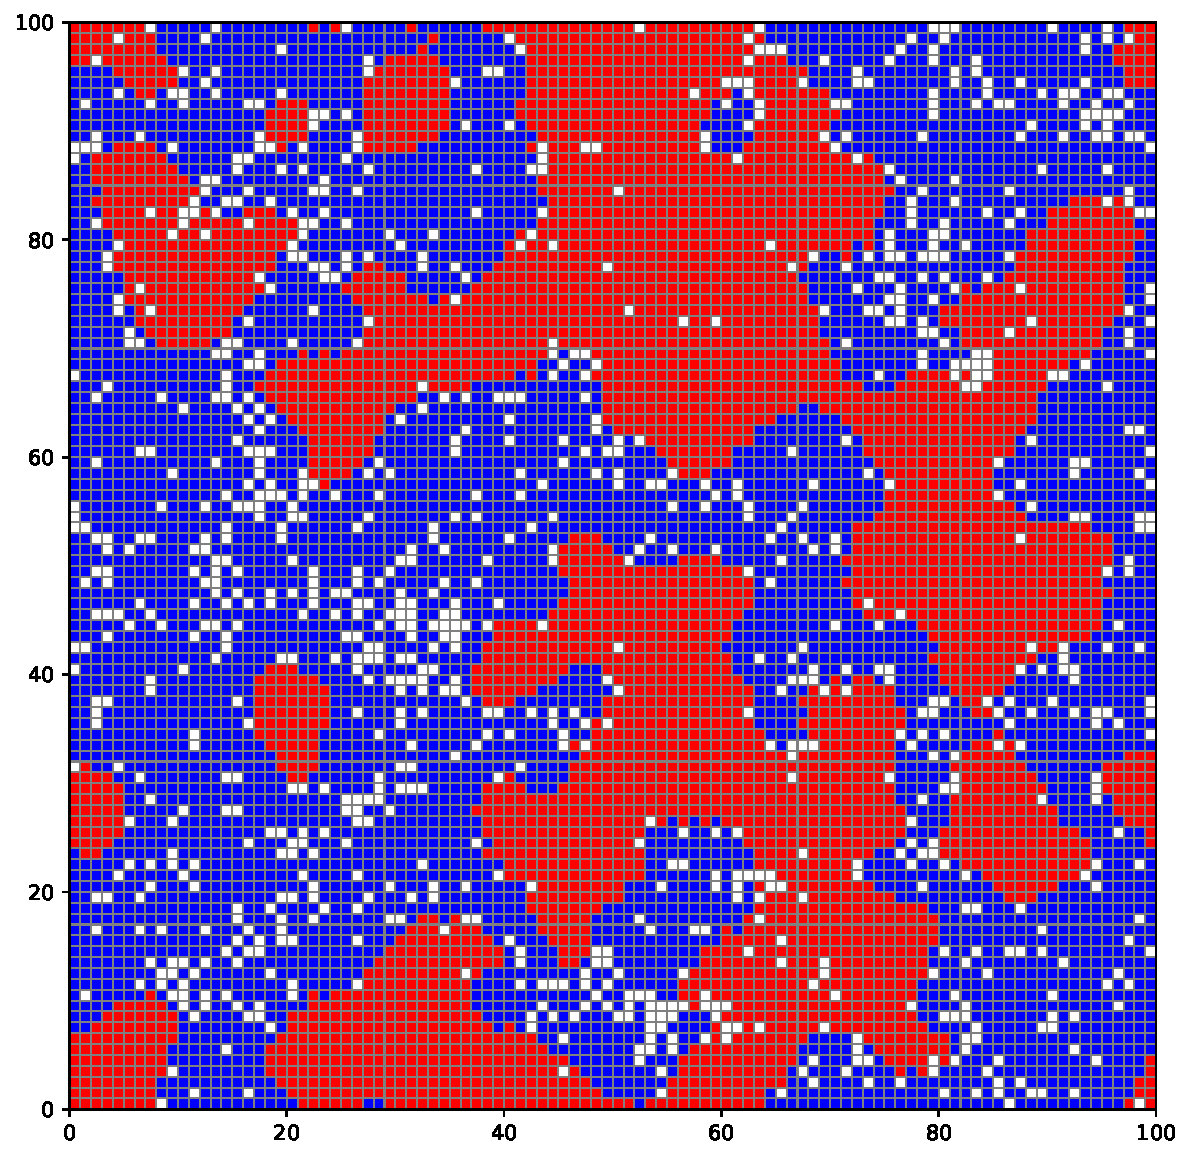
\includegraphics[width=\textwidth]{figs/schelling_model_0.4.pdf}	
	\end{subfigure}
    \begin{subfigure}{0.45\textwidth}	
	\centering
     \caption{"Gated" community, $1-\tau = 0.60$}
	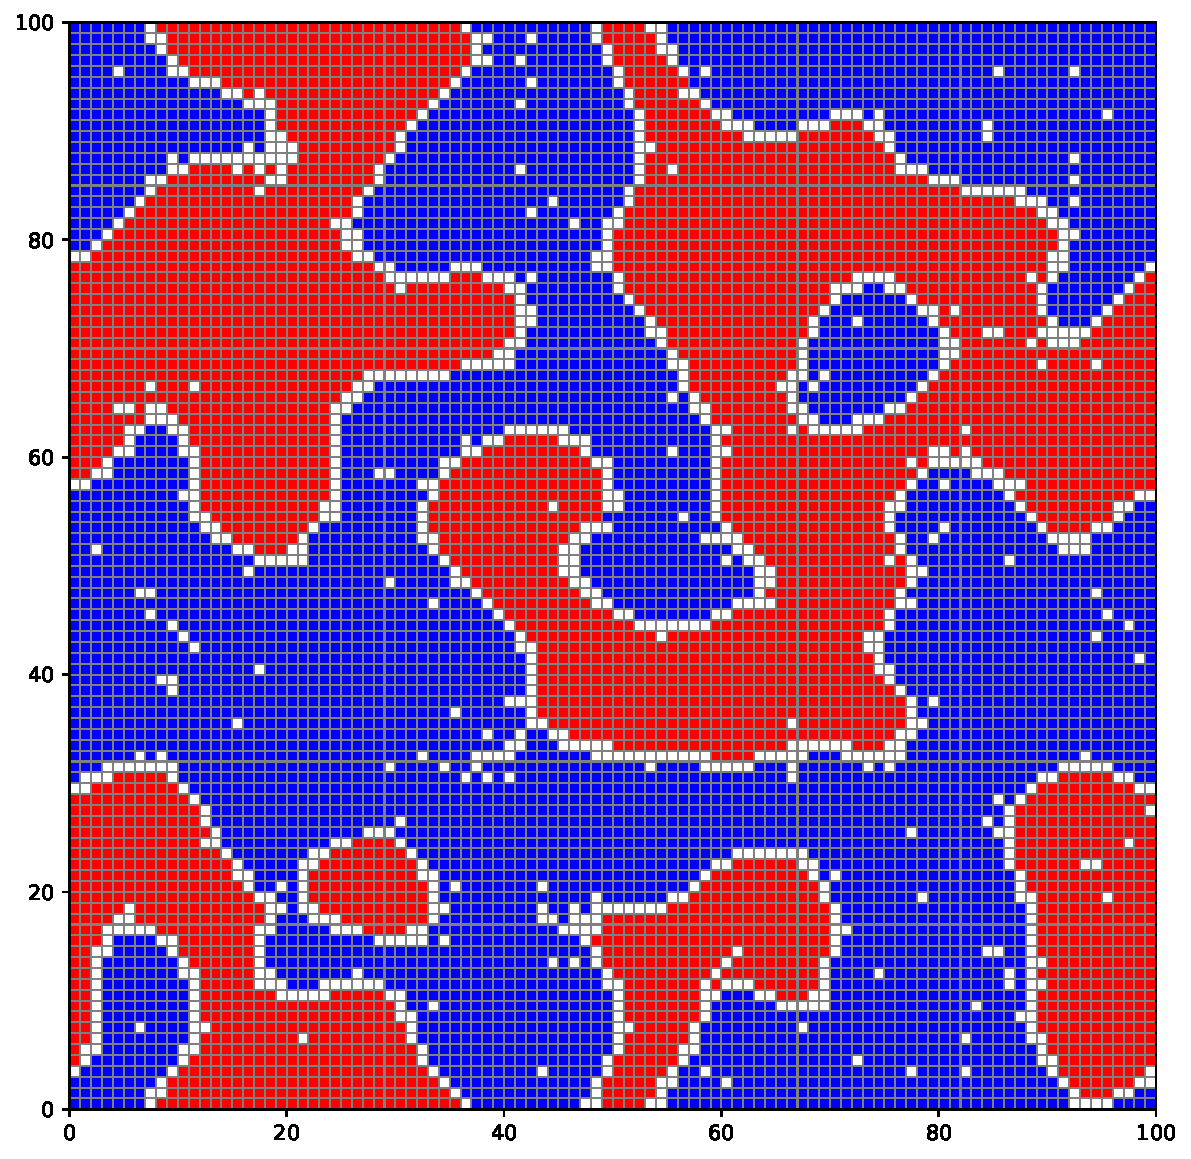
\includegraphics[width=\textwidth]{figs/schelling_model_0.6.pdf}	
	\end{subfigure}
\end{figure}

It is clear that the model predicts a segregated scenario for relatively mild preference parameters. Unsurprisingly, for sufficiently low levels of tolerances, one can observe fairly integrated societies. However, this pattern reverses once the tolerance parameter goes up, but not at levels one might expect. Even when agents are willing to accept up to 60 percent diverse neighbours ($1-\tau = 0.4$), we start to observe almost perfectly segregated societies.

...

\section{Datasets used}
\begin{table}[H]
    \centering
    \caption{Datasets}
    \begin{tabular}{l|p{0.6\linewidth}|c}
    \toprule
      Name & Notes & years \\
    \midrule
      BEF           & The basics, ID, AGE etc               & 1985-2024 \\
      BEFBOP        & Tracks adress changes over time. & 1986-2024 \\
      BEFADR        & Adress register. & 1971-2023 \\
      DAR(?)        & Danish Adress Registry. & 2017-2024 \\ 
      ETRS & (\textbf{NB!}) The "unique" coordinate dataset. & ?-?\\
      EJER & Historical house prices. & 1984-2023 \\
      EJVK & Dwelling valuations. & 1983-2023 \\
      AKM/RAS & (Un)employment. & 1976-2022 \\
      IND & Income, both wage and public transfers. & 1980-2022 \\
      UDDF & Education level. & 1974-2022 \\
      \hdashline
      KRAF(?)       & Crime registry (of court decisions). & 1980-2023\\
      KOTRE(?)      & Completed school grades               & 1970-2023 \\
    \bottomrule
    \end{tabular}
\end{table}

\section{Figures}
\label{sec:appendix_figs}
\begin{figure}[H]
    \centering
    \caption{Neighborhood population share by year}
    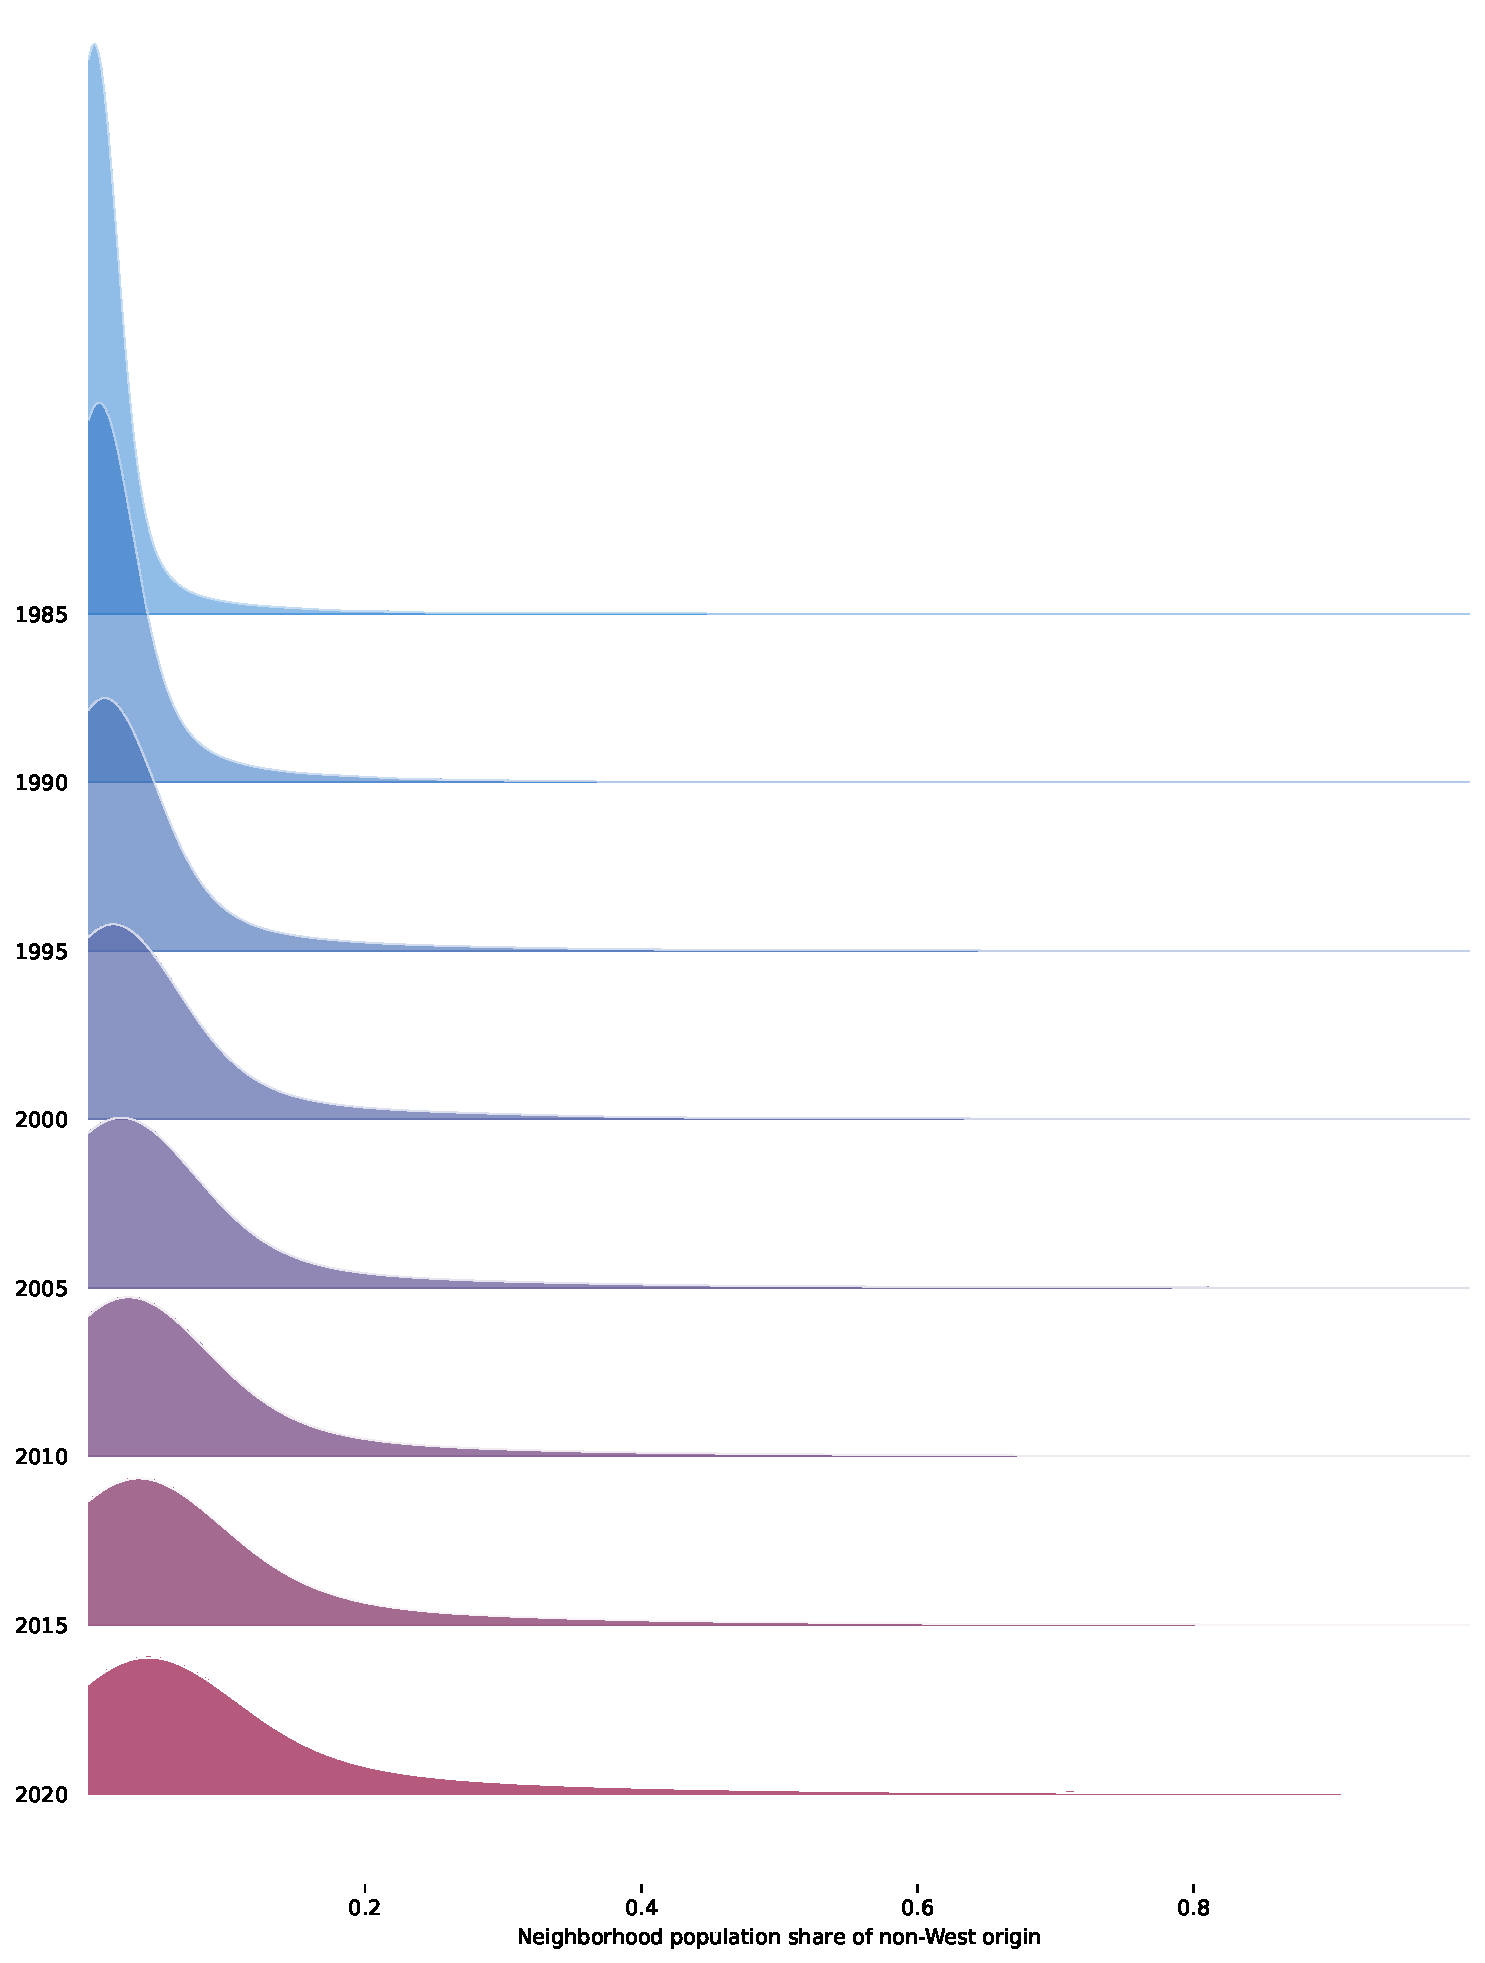
\includegraphics[width=0.7\linewidth]{figs/neighborhood_non_west_share_density_1985_2000.pdf}
        \begin{minipage}{.9\linewidth}
        \footnotesize \textit{Note}: Neighborhoods are derived from \href{https://www.nabolagsatlas.dk/}{Nabolagsatlas}. 
    \end{minipage}
\end{figure}

\begin{figure}[H]
    \centering
    \caption{K = 20 nearest }
    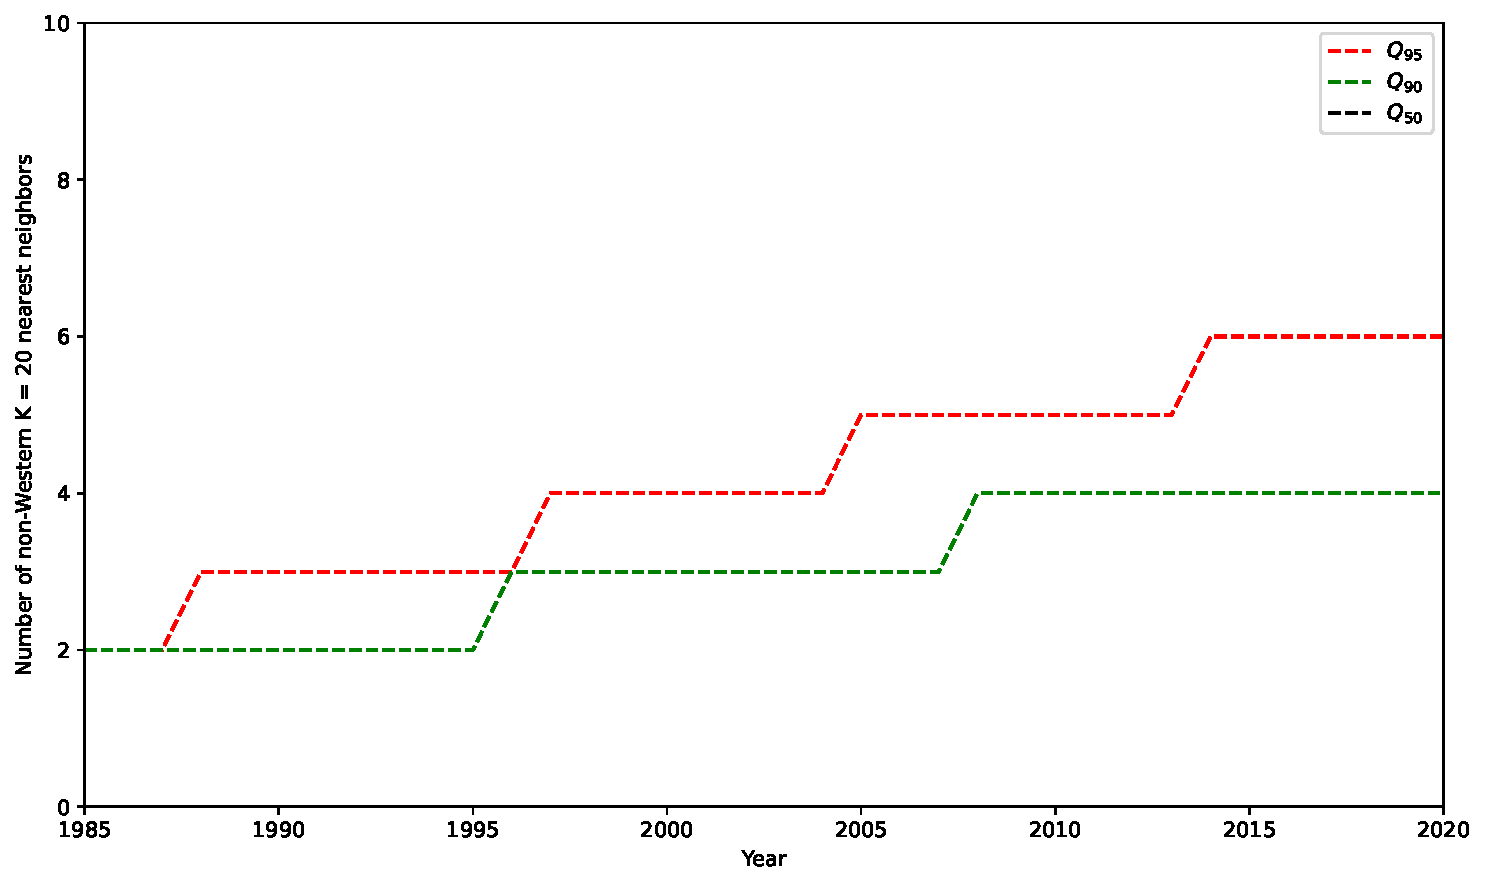
\includegraphics[width=0.7\linewidth]{figs/mix_non_west_pos_nn_quantiles_1985_2020.pdf}
        \begin{minipage}{.7\linewidth}
        \footnotesize \textit{Note}: Non-Western households refers to households where at least one household member is of non-Western origin.
    \end{minipage}
\end{figure}

\end{document}